\chapter{Introduzione}

Con l'avvento di internet e quindi dell'era digitale, durante gli ultimi decenni si è dovuto far fronte a molte minacce che riguardavano il mondo informatico. I malintenzionati sfruttano vulnerabilità di tutti i tipi, come ad esempio vulnerabilità che coinvolgono un componente informatico oppure che coinvolgono vulnerabilità di un programma e attraverso quest'ultimo prendere il controllo della macchina.
Negli ultimi anni però, c'è stato un incremento sostanziale delle truffe che hanno come obbiettivo quello di sfruttare la mancata attenzione da parte dell'utente finale al fine di mettere in atto la truffa.
Questo tipo di truffe è conosciuto con il nome di Phishing.\\
Con questa pratica, appunto, il malintenzionato cerca di ingannare la vittima convincendola a fornire informazioni personali, dati finanziari o codici di accesso, fingendosi un ente affidabile o una persona famosa.\\
Per commettere la pratica del phishing, spesso ci si avvale di un'altro tipo di cybercrime denominato domain squatting: Il cybersquatting è l'atto da parte del malintenzionato di appropriarsi di nomi di dominio che somigliano ai marchi commerciali più famosi o persone famose per effettuare il phishing.\\
Cercherò in questo articolo di esporre un sistema in grado di evitare che malintenzionati possano utilizzare domini internet (in particolare domini cybersquatting) per effettuare phishing. Generare potenziali domini di squatting in modo proattivo ci permette di identificarli ancora prima che possano essere utilizzati da malintenzionati per attacchi di phishing. SquatGAN è il prototipo iniziale di un sistema in grado di produrre questo sistema di generazione di domini. I risultati preliminari sono soddisfacenti ma non completi: quasi la totalità di essi sono domini typo squatting, i domini homographic squatting non vengono identificati in quanto il sistema di riconoscimento ottico dell'immagine non è stato ancora adattato per questo tipo di risultati (nel capitolo 4 sarà spiegato più in dettaglio).

\section{Lavoro correlato}
In questo articolo cercherò di emulare il comportamento di PishGan\cite{sern2020phishgan} il quale genera potenziali domini di squatting in modo pro-attivo utilizzando l'apprendimento automatico. Ciò che caratterizza il lavoro effettuato per PhishGan è il fatto di aver utilizzato come modello di rete neurale, una U-Net. Queste reti sono le più popolari per effettuare quella che viene chiamata "Image segmentation" (Segmentazione dell'immagine), il quale permette di partizionare l'immagine in regioni/segmenti per permettere una comprensione più semplice dell'immagine stessa (la figura \ref{fig:segmentation} mostra un esempio di segmentazione con due immagini diverse da cui si evidenziano le caratteristiche principali). Queste reti neurali vengono spesso usate in campo biomedico (ad esempio per la previsione del legame di una struttura proteica) e sono strutturate da due parti chiamate Encoder e Decoder. Nelle reti U-Net (figura \ref{fig:unet})\footnote[1]{https://www.frontiersin.org/articles/10.3389/fnins.2020.568614}, nel fronte di discesa, vengono apprese le features attraverso strati di convoluzione mentre nel fronte di salita (Decoder) vengono ricostruite le informazioni facendo convoluzione trasposta concatenando le features map nel corrispondente layer dell'Encoder.
Il concetto alla base di PhishGan è proprio questo, quello che andrò a sviluppare invece, sarà sempre un software di generazione di domini di squatting, ma utilizzando reti neurali convoluzionali generative (DCGAN).
\begin{figure}[!h]
  \centering
  \begin{minipage}[b]{\textwidth}
    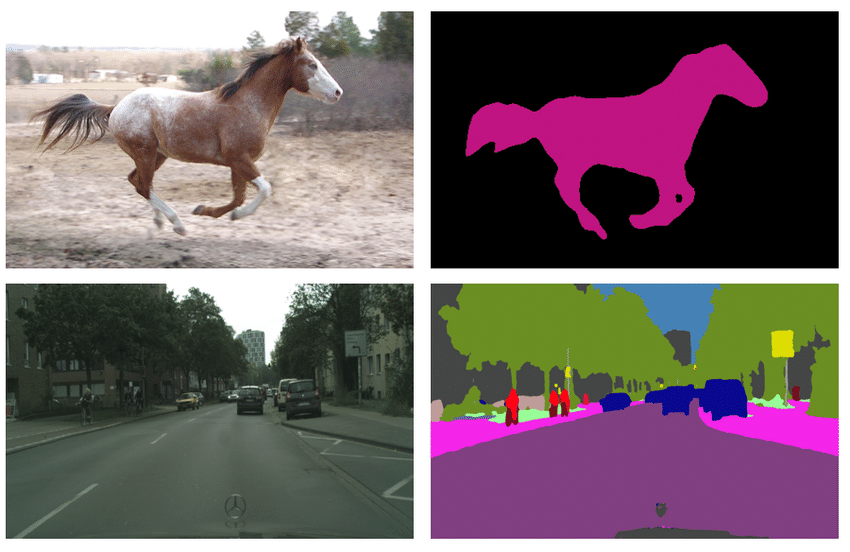
\includegraphics[width=\textwidth]{pictures/segmentation.png}
    \caption{IEsempio di image segmentation}
    \label{fig:segmentation}
  \end{minipage}
  \hfill
\end{figure}
\begin{figure}[!h]
  \centering
  \begin{minipage}[b]{\textwidth}
    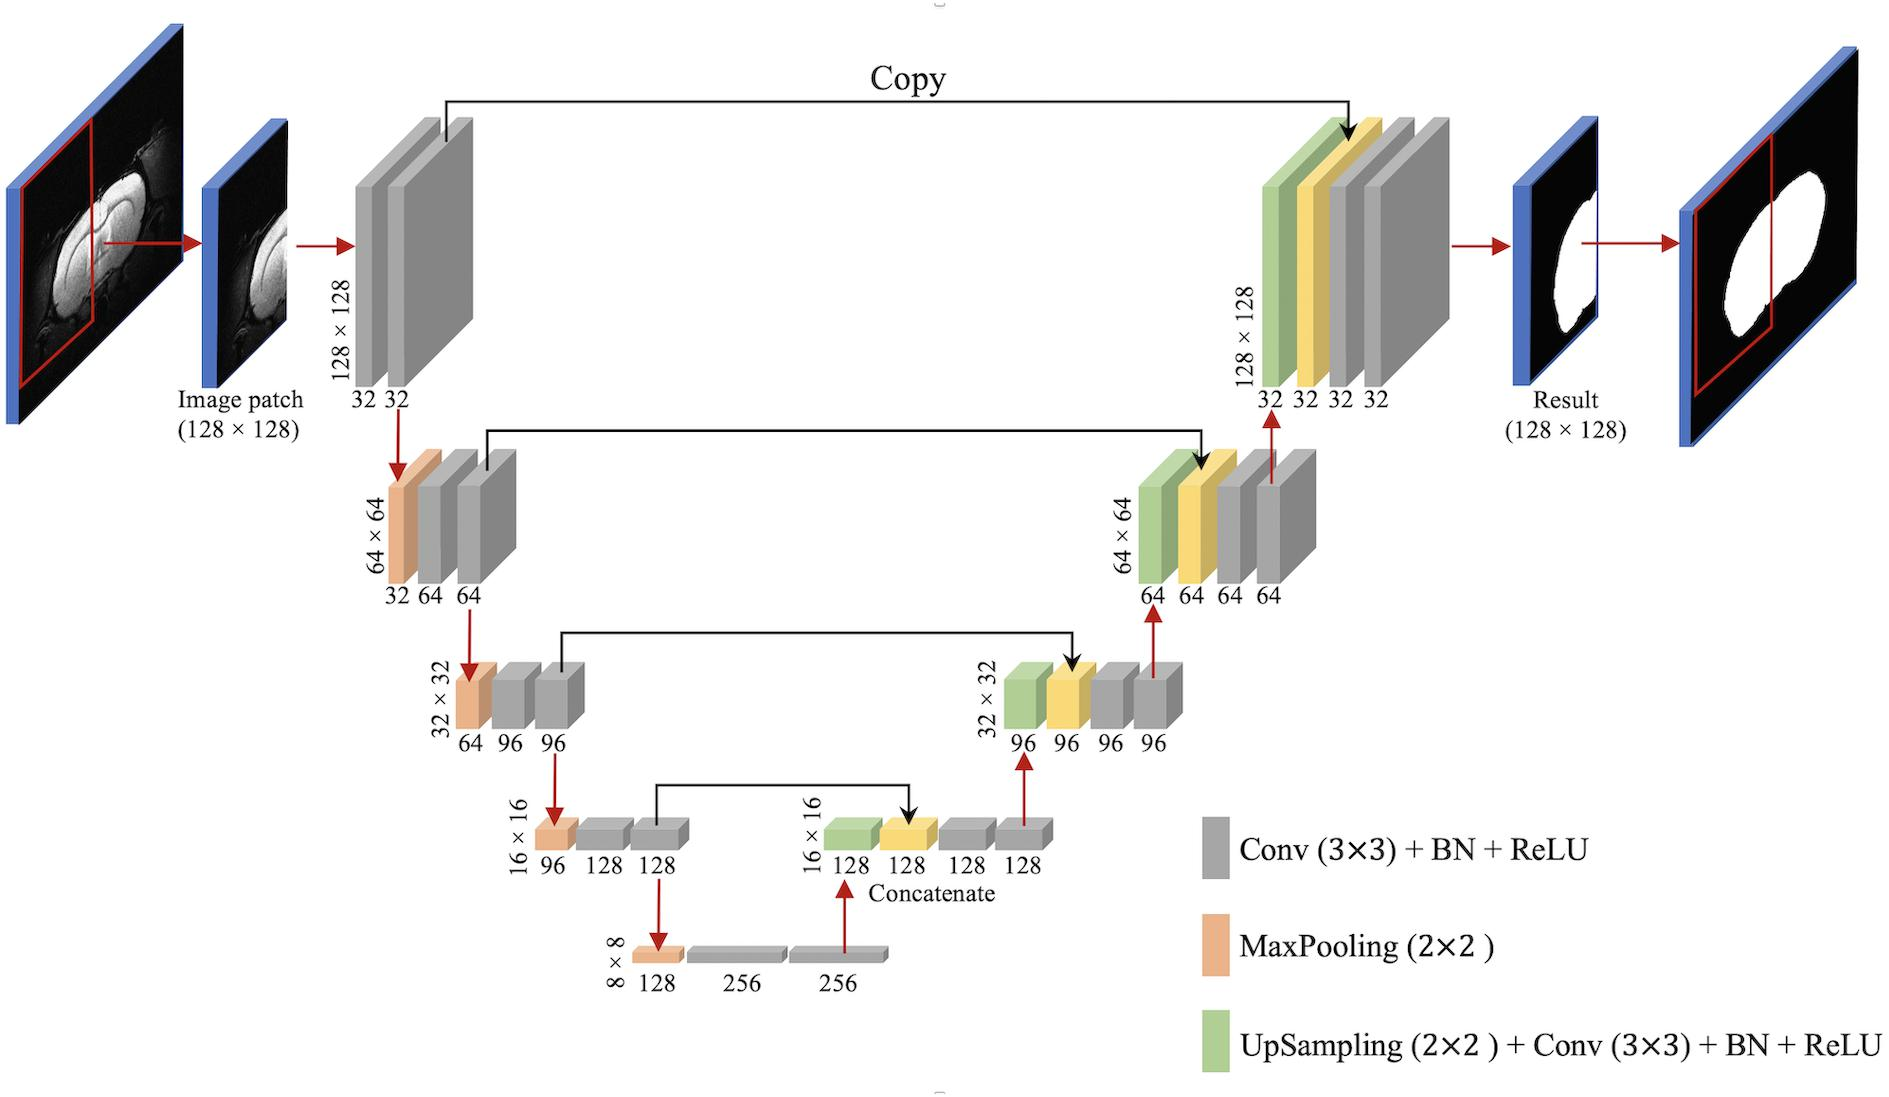
\includegraphics[width=\textwidth]{pictures/unet.jpg}
    \caption{Esempio di architettura U-Net ('U' perchè la forma che assume la rete assomiglia alla lettera 'U')}
    \label{fig:unet}
  \end{minipage}
  \hfill
\end{figure}
\section{Come è strutturato questo articolo}
Nella prima parte dell'articolo illustrerò contesti in cui può essere applicato il phishing e come viene usato insieme al cybersquatting per ingannare gli utenti al fine di rubare dati sensibili. Illustrerò con che strumento sarebbe possibile risolvere questo problema (utilizzando reti neurali generative) per poi concludere illustrando alcune applicazioni per la cybersecurity.\\
Nella seconda parte, illustrerò l'architettura utilizzata in SquatGAN mentre nell'ultima parte del documento illustrerò i risultati preliminari e come sono arrivato ad ottenere quest'ultimi.